% THIS IS SIGPROC-SP.TEX - VERSION 3.1
% WORKS WITH V3.2SP OF ACM_PROC_ARTICLE-SP.CLS
% APRIL 2009
%
% It is an example file showing how to use the 'acm_proc_article-sp.cls' V3.2SP
% LaTeX2e document class file for Conference Proceedings submissions.
% ----------------------------------------------------------------------------------------------------------------
% This .tex file (and associated .cls V3.2SP) *DOES NOT* produce:
%       1) The Permission Statement
%       2) The Conference (location) Info information
%       3) The Copyright Line with ACM data
%       4) Page numbering
% ---------------------------------------------------------------------------------------------------------------
% It is an example which *does* use the .bib file (from which the .bbl file
% is produced).
% REMEMBER HOWEVER: After having produced the .bbl file,
% and prior to final submission,
% you need to 'insert'  your .bbl file into your source .tex file so as to provide
% ONE 'self-contained' source file.
%
% Questions regarding SIGS should be sent to
% Adrienne Griscti ---> griscti@acm.org
%
% Questions/suggestions regarding the guidelines, .tex and .cls files, etc. to
% Gerald Murray ---> murray@hq.acm.org
%
% For tracking purposes - this is V3.1SP - APRIL 2009

\documentclass{edm_template}
\usepackage{multirow}
\usepackage{csquotes}
\usepackage{listings}
\usepackage{fixltx2e}
\usepackage{floatrow}
\usepackage{url}
\usepackage[font=small,skip=0pt]{caption}

\makeatletter
\def\@copyrightspace{\relax}
\makeatother
\setlength{\floatsep}{5pt}
\setlength{\textfloatsep}{4pt}
\setlength{\intextsep}{5pt}

\newcommand{\squishlist}{
 \begin{list}{$\bullet$}
 {
  \setlength{\itemsep}{0pt}
  \setlength{\parsep}{3pt}
  \setlength{\topsep}{3pt}
  \setlength{\partopsep}{0pt}
  \setlength{\leftmargin}{1.5em}
  \setlength{\labelwidth}{1em}
  \setlength{\labelsep}{0.5em} } }

\newcommand{\squishlisttwo}{
 \begin{list}{$\bullet$}
 {
  \setlength{\itemsep}{0pt}
  \setlength{\parsep}{0pt}
  \setlength{\topsep}{0pt}
  \setlength{\partopsep}{0pt}
  \setlength{\leftmargin}{2em}
  \setlength{\labelwidth}{1.5em}
  \setlength{\labelsep}{0.5em} } }

\newcommand{\squishend}{
  \end{list}  }

\begin{document}

\title{YouEDU: Addressing Confusion in MOOC Discussion Forums by Recommending Instructional Video Clips}
%\subtitle{[Extended Abstract]
%\titlenote{A full version of this paper is available as
%\textit{Author's Guide to Preparing ACM SIG Proceedings Using
%\LaTeX$2_\epsilon$\ and BibTeX} at
%\texttt{www.acm.org/eaddress.htm}}}
%
% You need the command \numberofauthors to handle the 'placement
% and alignment' of the authors beneath the title.
%
% For aesthetic reasons, we recommend 'three authors at a time'
% i.e. three 'name/affiliation blocks' be placed beneath the title.
%
% NOTE: You are NOT restricted in how many 'rows' of
% "name/affiliations" may appear. We just ask that you restrict
% the number of 'columns' to three.
%
% Because of the available 'opening page real-estate'
% we ask you to refrain from putting more than six authors
% (two rows with three columns) beneath the article title.
% More than six makes the first-page appear very cluttered indeed.
%
% Use the \alignauthor commands to handle the names
% and affiliations for an 'aesthetic maximum' of six authors.
% Add names, affiliations, addresses for
% the seventh etc. author(s) as the argument for the
% \additionalauthors command.
% These 'additional authors' will be output/set for you
% without further effort on your part as the last section in
% the body of your article BEFORE References or any Appendices.

\numberofauthors{4} %  in this sample file, there are a *total*
% of EIGHT authors. SIX appear on the 'first-page' (for formatting
% reasons) and the remaining two appear in the \additionalauthors section.
%
\author{
% You can go ahead and credit any number of authors here,
% e.g. one 'row of three' or two rows (consisting of one row of three
% and a second row of one, two or three).
%
% The command \alignauthor (no curly braces needed) should
% precede each author name, affiliation/snail-mail address and
% e-mail address. Additionally, tag each line of
% affiliation/address with \affaddr, and tag the
% e-mail address with \email.
%
% 1st. author
\alignauthor Akshay Agrawal \\
       \affaddr{Stanford University} \\
       \email{akshayka@cs.stanford.edu}
\alignauthor Jagadish Venkatraman \\
       \affaddr{Stanford University} \\
       \email{jagadish@cs.stanford.edu}
\alignauthor Shane Leonard \\
       \affaddr{Stanford University} \\
       \email{shanel@stanford.edu}
\and
\alignauthor Andreas Paepcke \\
       \affaddr{Stanford University} \\
       \email{paepcke@cs.stanford.edu}
% \and   use '\and' if you need 'another row' of author names
} % \author
\date{9 February 2015}
% Just remember to make sure that the TOTAL number of authors
% is the number that will appear on the first page PLUS the
% number that will appear in the \additionalauthors section.

\maketitle
\begin{abstract}
In Massive Open Online Courses (MOOCs), struggling learners often seek help by
posting questions in discussion forums. Unfortunately, given the large volume of discussion in MOOCs, instructors may overlook these learners' posts,
detrimentally impacting the learning process and exacerbating attrition. In this paper, we present YouEDU, an instructional aid that automatically detects and addresses confusion in forum posts. Leveraging our Stanford MOOCPosts corpus, we train a set of classifiers to classify forum posts across multiple dimensions. In particular, classifiers that target sentiment, urgency, and other descriptive variables inform a single classifier that detects confusion. We then employ information retrieval techniques to map confused posts to minute-resolution clips from course videos; the ranking over these clips accounts for textual similarity between posts and closed captions. We measure the performance of our classification model in multiple educational contexts, exploring the nature of confusion within each; we also evaluate the relevancy of materials returned by our ranking algorithm. Experimental results demonstrate that YouEDU achieves both its goals, paving the way for intelligent intervention systems in MOOC discussion forums.
\end{abstract}

%% A category with the (minimum) three required fields
%\category{H.4}{Information Systems Applications}{Miscellaneous}
%%A category including the fourth, optional field follows...
%\category{D.2.8}{Software Engineering}{Metrics}[complexity measures, performance measures]
%
%\terms{Theory}

\section{Introduction}
\label{sec:intro}

During recent years, many universities have experimented with online delivery of their courses to the public. Hundreds of thousands of learners across the world have taken advantage of these Massive Open Online Courses (MOOCs). While MOOCs are certainly more accessible than physical classes, the virtual domain brings with it its own challenges.

Lacking physical access to teachers and peer groups, learners resort to discussion forums in order to both build a sense of belonging and to better understand the subject matter at hand. Indeed, these forums could in theory be rich reflections of learner affect and academic progress. But, with MOOC enrollments so high, forums can seem unstructured and might even inhibit, rather than promote, community \cite{community}. It becomes intractable for instructors to effectively monitor and moderate the forums. Learners seeking to clarify concepts might not get the attention that they need, as the greater sea of discussion drowns out their posts. The lack of responsiveness in forums might even push learners to drop out of courses altogether \cite{wen2015confusion}.

The unattended, confused learner might revisit instructional videos in order to solidify his or her understanding. Yet video, a staple of MOOCs, is tyrannically linear. No table of contents or hyperlinks are available to access material in an organized fashion. Often presented with more than one hundred ten-to-fifteen-minute videos, learners might become discouraged when they realize that they will have to re-view footage to patch holes in their knowledge.

We concerned ourselves with solving the problems related to discussion forums and videos that arise when confusion goes unaddressed. In this paper, we present YouEDU, a unified pipeline that automatically classifies forum posts across multiple dimensions, staging intelligent interventions when appropriate.  In particular, for those posts in which our classifier detects confusion, our pipeline recommends a ranked list of one-minute-resolution video snippets that are likely to help address the confusion. These recommendations are computed by using subsets of post contents as queries into closed caption files. That the snippets be short is important; \cite{Guo:2014:VPA:2556325.2566239} found that, regardless of video length, learners' median engagement time with videos did not exceed six minutes. Individual learners may watch beyond the minute we recommend, should they wish. 

In order to enable YouEDU's classification phase, we hired consultants to tag 30,000 posts from three categories of Stanford MOOCs: Humanities and Sciences, Medicine, and Education. The set, dubbed the Stanford MOOCPosts Dataset, is available to researchers on request \cite{stanfordMOOCPosts}. Besides describing the extent of confusion, each entry in the MOOCPosts set indicates whether a particular post was a {\em question}, an {\em answer}, or an {\em opinion}, and gauges the post's {\em sentiment} and {\em urgency} for an instructor to respond. In detecting confusion, our classifier takes into account the predictions of five other constituent classifiers, one for each of the variables (save confusion itself) encoded in our dataset.

The online teaching platforms that Stanford uses to distribute its public courses gather tracking log data comprising hundreds of millions of learner actions. We use a subset of these data as features for our confusion classification. Some of these data are also available in anonymized form to researchers upon request \cite{stanfordDataApps}. Until very recently, the data requisite for our classification approach---the MOOCPosts corpus and this additional metadata---simply did not exist. 

The remainder of this paper is organized as follows. We examine
related work in Section~\ref{sec:relWork}, present the MOOCPosts corpus in
Section~\ref{sec:MOOCPosts}, and sketch the architecture of YouEDU in
Section~\ref{sec:arch}.  In Sections~\ref{sec:confusionDetection} and
\ref{sec:clipRecommendation} we detail, evaluate, and discuss YouEDU's 
classification and recommendation phases. We close with a section on
future work, and a conclusion.

\section{Related Work}
\label{sec:relWork}

Stephens-Martinez, et al. \cite{Stephens-Martinez:2014:MMI:2556325.2566246} find that MOOC instructors highly value understanding the activity in their discussion forums. The role of instructors in discussion forums is investigated in \cite{Tomkin:2014:PMU:2556325.2566245}, which finds that learners' experiences are not appreciably affected by the presence or absence of (sparse) instructor intervention. The study did not, however, allow for instructors to regularly provide individual feedback to learners. Instructors interviewed in \cite{hollands2014moocs} stress the need for better ways to navigate MOOC forums, and one instructor emphasizes in particular the benefits to be reaped by using natural language processing to reorganize forums. 

Wen, et al. \cite{wen2014sentiment} explore the relationship between attrition and sentiment, using a sentiment lexicon derived from movie reviews. Yang, et al. \cite{wen2015confusion} conduct an investigation into the relationship between attrition and confusion. While \cite{wen2015confusion} also presents a classifier for confusion, our classification approach differs from theirs in that it operates on a larger dataset and uses a different set of features, including those generated by other classifiers. Chaturvedi, et al. \cite{chaturvedipredicting} predict instructor intervention patterns in forums. Our work is subtly different in that we predict posts that coders---who carefully read every post in a set of courses---deemed to be urgent, rather than learning from posts that the instructors themselves had responded to. The classification of documents by opinion and sentiment is treated in \cite{song2007opinion} and \cite{binali2009new}. 

Yang, et al. \cite{yang2014forum} propose a recommendation system that matches learners to threads of interest, while Guy, et al. \cite{shaniedurank} devise an algorithm to personalize the questions presented to learners. The need for intervention systems to address confusion in particular is highlighted in \cite{wen2015confusion}. Closed caption files were used in the Informedia project \cite{Wactlar:1996:IAD:619007.620445} to index into television news shows. To the best of our knowledge, the same has not been done in the context of MOOCs. 


\section{The Stanford MOOCPosts Corpus}
\label{sec:MOOCPosts}

Given that no requestable corpus of tagged MOOC discussion forum posts existed prior to our research, we set out to create our own. The outcome of our data compilation and curation was the Stanford MOOCPosts Dataset: a corpus composed of 29,604 anonymized learner forum posts from eleven Stanford University public online classes. Available on request to academic researchers, the MOOCPosts dataset was designed to enable computational inquiries into MOOC discussion forums.

Each post in the MOOCPosts dataset was scored across six dimensions---confusion, sentiment, urgency, question, answer, and opinion---and subsequently augmented with additional metadata.


\subsection{Methodology: Compiling the Dataset}
We organized the posts by course type into three groups: Humanities/Sciences, Medicine, and Education, with 10,000, 10,002, and 10,000 entries, respectively. Humanities/Sciences contains two economics courses, two statistics courses, a global health course, and an environmental physiology course; Medicine contains two runs of a medical statistics course, a science writing course, and an emergency medicine course; Education contains a single course, \emph{How to Learn Math}. 

Each course set was coded by three independent, paid oDesk coders. That is, three triplets of coders each worked on one set of 10,000 posts. No coder worked on more than one course set. Each coder attempted to code every post for his or her particular set. All posts with malformed or missing scores in at least one coder's spreadsheet were discarded. This elision accounts for the difference between the 29,604 posts in the final set, and the original 30,002 posts.

Coders were asked to score their posts across six dimensions:
\begin{itemize}
%\squishlist
\vspace{-15pt}
       \setlength\itemsep{0.05em}
       \item Question: Does this post include a question?
       \item Opinion: Does this post include an opinion, or is its subject matter wholly factual?
       \item Answer: Is this post an answer to a learner's question?
       \item Sentiment: What sentiment does this post convey, on a scale of 1 (extremely negative) to 7 (extremely positive)? A score of 4 indicates neutrality.
       \item Urgency: How urgent is it that an instructor respond to this post, on a scale of 1 (not urgent at all) to 7 (extremely urgent)? A score of 4 indicates that instructors should respond only if they have spare time.
       \item Confusion: To what extent does this post express confusion, or the lack thereof, on a scale of 1 (expert knowledge) to 7 (extreme confusion)? A score of 4 indicates neither knowledge nor confusion.
\end{itemize}
%\squishend
\vspace{-15pt}
Coders were given examples of posts in each category. The following was an example of an extremely urgent post:

\vspace{-14pt}
\begin{displayquote}
\emph{The website is down at the moment
       https:\\//class.stanford.edu/courses/Engineering/\\Networking/Winter2014/courseware
       seems down and I'm not able to submit the Midterm. Still have
       the "Final Submit" button on the page, but it doesn't work. Are
       the servers congested? 
       thanks anyway}
\end{displayquote}
\vspace{-14pt}

And

\vspace{-14pt}
\begin{displayquote}
\emph{Double colons "::"  expand to longest possible 0's  
       If the longest is 0, will  the address be considered valid ?  (
       even if it doesn't make sense and there is no room for adding
       0's) 
       Can someone please answer ?
       Thanks in advance}
\end{displayquote}
\vspace{-14pt}

was given as an example of a post that was both confused (6.0) and urgent (5.0).

We created three gold sets from the coders' scores, one for each course type. We computed inter-rater reliability using Krippendorff's Alpha \cite{hayes2007answering}. For a given post and Likert variable, the post's gold score was computed as an unweighted average of the scores assigned to it by the subset of two coders who expressed the most agreement on that particular variable. Gold scores for binary variables were chosen by majority votes across all three coders. We refer readers to our write-up in \cite{stanfordMOOCPosts} for a more detailed treatment of our procedure and the complete inter-rater reliability results.


\subsection{Discussion}
We found significant correlations between confusion and the other five variables. In the humanities and medicine course sets, confusion and urgency were correlated with a Pearson's correlation coefficient of 0.657 and 0.485, respectively. In all three subdivisions of the dataset, confusion and the question variable were positively correlated (0.623, 0.459, and 0.347), while the sentiment, opinion, and answer variables were negatively correlated with confusion. Table \ref{table:correlations} reports the entire set of correlations.

That questions and confusion were positively correlated supports the finding in \cite{wilson1989learning} that confusion is often communicated through questions. The negative correlations can be understood intuitively. Confusion might turn into frustration and negative sentiment; as discussed in \cite{liu2013sequences}, confusion and frustration sometimes go hand-in-hand. If a learner is opining on something, then it seems less likely that he or she is discussing course content. And we would hope that learners providing answers are not themselves confused.

\begin{table}
       \centering
       \begin{tabular}{|c|c|c|c|}
       \hline
          & Humanities & Medicine & Education \\ \hline
        Urgency   & 0.657                & 0.485              & 0.000* \\ \hline
        Sentiment & -0.171                & -0.098             & -0.134 \\ \hline
        Opinion   & -0.193                & -0.097             & -0.297 \\ \hline
        Answer    & -0.257                & -0.394             & -0.106  \\ \hline
        Question  & 0.623                & 0.459              & 0.347  \\ \hline
       \end{tabular}
       \vspace{-5pt}
       \caption{\textnormal{
       Correlations with Confusion. The urgency and question variables are strongly correlated with confusion. All correlations, save the one denoted by *, were significant, with p-values < 0.01.
       }} 
       \label{table:correlations} % is used to refer this table in the text
\end{table}


% TODO: Perhaps fold this into the introduction.
\section{YouEDU: Detect and Recommend}
\label{sec:arch}

YouEDU\footnote{Our entire implementation is open-source.} is an intervention system that recommends educational video clips to learners. Figure \ref{figure:architecture} illustrates the key steps that comprise YouEDU. YouEDU takes as input a set $P$ of forum posts, processing them in two distinct phases: (I) detection and (II) recommendation. In the first phase, we apply a classifier to each post in $P$, outputting a subset $P_{c}$ consisting of posts in which the classifier detected confusion. The confusion classifier functions as a \emph{combination} classifier in that it combines the predictions from classifiers trained to predict other post-related qualities (Section~\ref{sec:confusionDetection}).

The second phase takes $P_{c}$ as input and, for each confused post $P_{m} \in P_{c}$, outputs a ranked list of educational video snippets that address the object of confusion expressed in $P_{m}$. In particular, for a given post, the recommender produces a ranking across a number of one-minute video clips by computing a similarity metric between the post and closed caption sections. In an online system, of course, learners may choose to watch beyond the end of the one-minute snippet---the snippets effectively function as a video index.
\begin{figure}[htp]
       \centering
       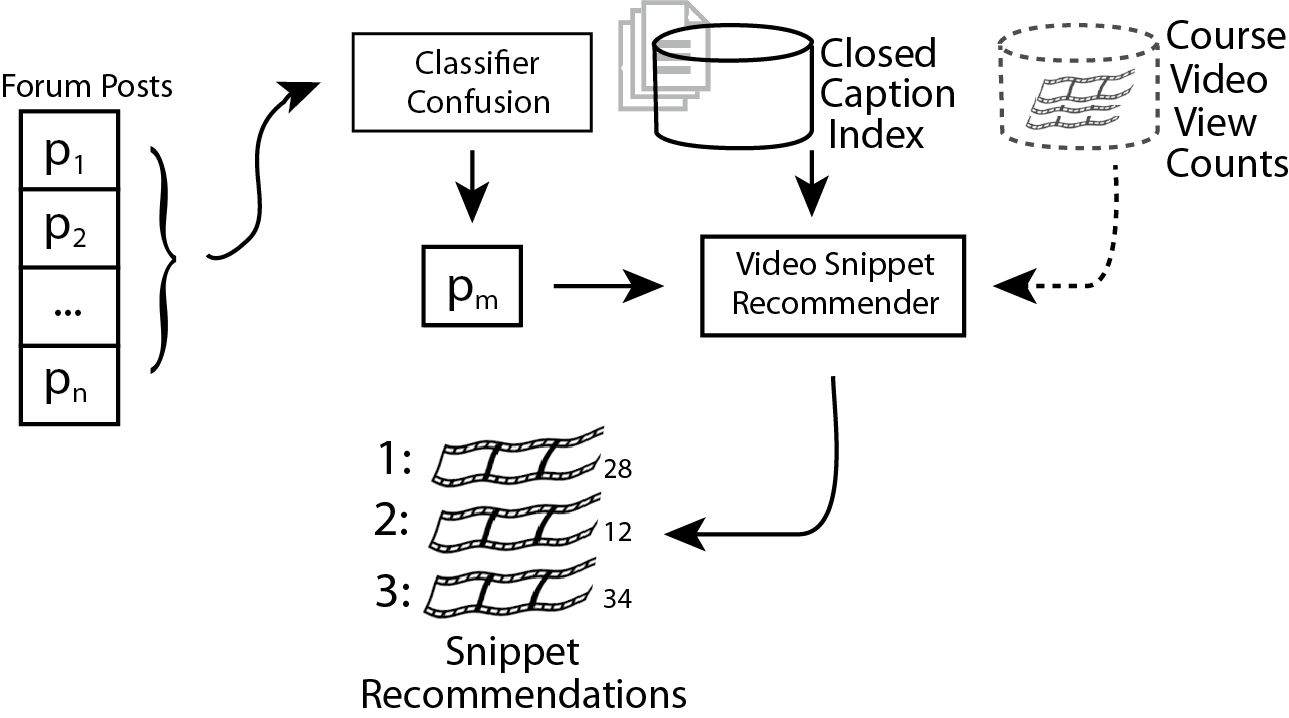
\includegraphics[width=1.0\textwidth]{../Figs/youEduArch.png}
       \caption{\textnormal{YouEDU Architecture. YouEDU 
           consists of two phases: post classification and video
           snippet recommendation. The dotted-line module is under
           construction (see Section~\ref{sec:futureWork}).}}
       \label{figure:architecture}
\end{figure}

\section{Phase I: Detecting Confusion}
\label{sec:confusionDetection}

% TODO: Cite
We frame the problem of detecting confusion as a binary one. Posts with a confusion rating greater than four in the MOOCPosts dataset fall into the ``confused'' class, while all other posts fall into the ``not confused'' class. We craft a rich feature space that fully utilizes the data available in our MOOCPosts dataset, choosing logistic regression with $l_{2}$ regularization as our model.

\subsection{Feature Space and Model Design}
Our feature space is composed of three types of inputs, those derived from the post body, post metadata, and other classifiers. The confusion classifier we train functions as a combining layer that folds in the predictions of other classifiers; these classifiers are trained to predict variables correlated with confusion. We expand upon each type of input here.


\subsubsection{Bag-of-Words}
We take the bag-of-words approach in representing documents, or forum posts. The unigram representation, while simple, pervades text classification and often achieves high performance \cite{boulis2005text}. We employ $l_{2}$ regularization to prevent overfitting, a risk that is aggravated when the dimension of the feature space exceeds the training set size \cite{Ng:2004:FSL:1015330.1015435}.

Each document is represented in part as a vector of indicator variables, one for each word that appears in the training data---the $i$-th indicator is 1 if the $i$-th word in the vocabulary is present in the document, otherwise. A word is defined as either a sequence of one or more alphanumeric characters or a single punctuation character (one of \{. , ; ! ?\}). 

Documents are pre-processed before they are mapped to vectors. We prune out stop words, using a subset of the stop word list published by the Information Retrieval Group at the University of Glasgow \cite{glasgow}. Removed words include, but are not limited to, interrogatives, words that identify the self (``I'', ``my''), verbs indicating ability or the lack thereof, negative words (``never'', ``not''), and certain conjunctions (``yet'', ``but''). We ignore alphabetic case and collapse numbers, \LaTeX\ equations, and URLs into three unique words.


\subsubsection{Post Metadata}
The feature vector derived from unigrams is augmented with post metadata, including: 
\vspace{-15pt}
\begin{itemize}
%\squishlist
\setlength\itemsep{0.05em}
       \item The number of up-votes accumulated by the post. We rationalized that learners might express interest in posts that voiced confusion that they shared. 
       \item The number of reads garnered by the post's thread.
       \item Whether the poster elected to appear anonymous to his or her peers or to the entire population. It has been shown that anonymity in educational discussion forums enables learners to ask questions without fear of judgement \cite{freeman2004student}, and our dataset demonstrates a strong correlation between questions and confusion.
       \item The poster's grade in the class at the time of post submission, where ``grade'' is defined as the number of points earned by the learner (e.g., by correctly answering quiz questions) divided by the number of points possible. The lower the grade, we hypothesized, the more likely the learner might be confused.
       \item The post position---most likely, we hypothesized, learners seeking help will create new threads.
\end{itemize}
%\squishend


\subsubsection{Classifier Combination}
In Section~\ref{sec:MOOCPosts}, we demonstrated that confusion is significantly correlated with questions, answers, urgency, sentiment and opinion. As such, in predicting confusion, we take into account the predictions of five distinct classifiers, one for each of the aforementioned variables. We use the fine-grained method of combining classifiers in which the outputs of several classifiers are fed as input to a \emph{combination function} \cite{bennett2005combination}. In our case, the combination function is itself a classifier.

For a given train-test partition, let $D_{train}$ be the training set and $D_{test}$ be the test set. Let $H_{q}$, $H_{a}$, $H_{o}$, $H_{s}$, and $H_{u}$ be classifiers for the question, answer, opinion, sentiment, and urgency variables, respectively. We call these classifiers \emph{constituent} classifiers. Each constituent is trained on $D_{train}$, taking as input bag-of-words and post metadata features.

Let $H_{c}$, a classifier for confusion, be our combination function. Like the constituent classifiers, $H_{c}$ is trained on $D_{train}$ and takes as input bag-of-words and metadata features. Unlike the constituents, $H_{c}$ also treats the ground-truth labels for the question, answer, opinion, sentiment, and urgency variables as features. When testing $H_{c}$ on an example $d \in D_{test}$, the constituent classifiers each output a prediction for $d$. These five predictions---and not the ground-truth values---are appended to the bag-of-words and metadata features derived from $d$. The resulting vector is given as input to $H_{c}$, which then predicts $d$'s confusion class.

A few subtleties: $H_{s}$ uses an additional metadata feature that the other classifiers do not---the number of negative words (e.g., ``not'', ``cannot'', ``never'', etc.). $H_{q}$, $H_{a}$, $H_{u}$, and $H_{c}$ treat the number of question marks as an additional feature, given the previously presented correlations; \cite{wen2015confusion} also used question marks in predicting confusion. And while $H_{q}$, $H_{a}$, and $H_{o}$ are by nature binary classifiers, $H_{s}$ and $H_{u}$ are multi-class. They predict values corresponding to negative (score $< 4$), neutral (score $= 4$), and positive (score $> 4$), providing $H_{c}$ with somewhat granular information. Going forward, we refer to the confusion classifier that uses all the features
described in this section as the \emph{combined} classifier. 

\subsection{Evaluation and Discussion}
In this section, we evaluate and interpret the performance of the combined classifier in contrast to confusion classifiers with pared-down feature sets, reporting insights gleaned about the nature of confusion in MOOCs along the way. 

\begin{table*}[htp!]
    \centering
    \begin{tabular}{|c|c c c|c c c|c|}
    \hline
    \multirow{2}{*}{Course Set} & \multicolumn{3}{c|}{Not Confused} & \multicolumn{3}{c|}{Confused}  & \multirow{2}{*}{Kappa} \\ \cline{2-7}
                                &  Precision & Recall & $F_{1}$     &  Precision & Recall & $F_{1}$  &       \\ \hline
    Humanities                  & 0.898      & 0.943    & 0.919     & 0.778      & 0.642  & 0.700    & 0.621  \\ \hline
    Medicine                    & 0.924      & 0.946    & 0.935     & 0.699      & 0.589  & 0.627    & 0.564  \\ \hline

    \end{tabular}
    \vspace{-5pt}
    \caption{\textnormal{
       Combined Confusion Classifier Performance, Course Sets.
    }} % title of Table
    \label{table:confusion_sets} % is used to refer this table in the text
\end{table*}

We quantify performance primarily using two metrics: $F_{1}$ and Cohen's Kappa. We favor the Kappa over accuracy because the former accounts for chance agreement \cite{cohen1960coefficient}. Unless stated otherwise, reported metrics represent an average over 10 folds of stratified cross-validation. 

Table \ref{table:confusion_sets} presents the performance of the combined classifier on the humanities and medicine course sets. As mentioned in Section~\ref{sec:MOOCPosts}, both sets are somewhat heterogeneous collections of courses, with a total of nearly 10,000 posts in each set. In our dataset, not-confused posts (that is, posts with a confusion score of at most 4) outnumber confused ones---only 23\% of posts exhibit confusion in the humanities course set, while 16\% exhibit confusion in the medicine course set.


\subsubsection{The Language of Confusion Across Courses}

\begin{table*}
       \centering
       \begin{tabular}{|c|c|c|c|c|}
       \hline
       Course                         & \# Posts (\% Confused) & $F_{1}$: Not Confused & $F_{1}$: Confused & Kappa \\ \hline
       Managing Emergencies              & 279 (18\%)                         & 0.963                 & 0.771             & 0.741 \\ \hline
       Statistical Learning              & 3,030 (30\%)                        & 0.909                 & 0.767             & 0.677 \\ \hline
       Economics 1                       & 1,583 (23\%)                     & 0.933                 & 0.741             & 0.675 \\ \hline
       Statistics in Medicine (2013)     & 3,320 (21\%)                         & 0.916                 & 0.671             & 0.589 \\ \hline
       Women's Health                    & 2,141 (15\%)                         & 0.933                 & 0.506             & 0.445 \\ \hline
       How to Learn Math                 & 9,878 (6\%)                        & 0.970                 & 0.383             & 0.359 \\ \hline
       \end{tabular}
       \vspace{-5pt}
       \caption{\textnormal{
       Combined Confusion Classifier Performance, Individual Courses. Our classifier performed best on courses whose discourse was characterized by technical diction, like statistics or economics. In courses like \emph{How to Learn Math} that facilitated open-ended and somewhat roaming discussions, our model found it more difficult to implicitly define confusion. 
       }} % title of Table
       \label{table:confusion_courses} % is used to refer this table in the text
\end{table*}

Table \ref{table:confusion_courses} presents the performance of the combined classifier on select courses, sorted in descending order by Kappa. Our classifier performed best on courses that traded in highly technical language. Take, for example, the following post that was tagged as confused from \emph{Managing Emergencies}, the course on which our classifier achieved its highest performance (Kappa = 0.741):

\vspace{-10pt}
\begin{displayquote}
\emph{At what doses is it therapuetic for such a patient because at high doses it causes vasoconstrition through alpha1 interactions, while at low doses it causes dilation of renal veins and splachinic vessels.}
\end{displayquote}
\vspace{-10pt}

The post is saturated with medical terms. A vocabulary so technical and esoteric is likely only used when a learner is discussing or asking a question about a specific course topic. Indeed, inspecting our model's weights revealed that ``systematic'' was the $11^{th}$ most indicative feature for confusion (odds ratio = 1.23) and ``defibrillation'' was the $15^{th}$ (odds ratio = 1.22). Similarly, in \emph{Statistical Learning}, ``solutions'' was the sixth most indicative feature (odds ratio = 1.75), and ``predict'' was the ninth (odds ratio = 1.65).

A glance at Table \ref{table:confusion_courses} suggests that our classifier's performance degrades as the discourse becomes less technical. Posts like the following were typical in \emph{How to Learn Math}, an education course about the pedagogy of mathematics:

\vspace{-10pt}
\begin{displayquote}
\emph{I am not sure if I agree with tracking or not.  I like teaching children at all levels ...  In a normal class setting the lower level learners can learn from the higher learners and vice versa.  Although I do find it very hard to find a middle ground. There has to be an easier way.}
\vspace{-10pt}
\end{displayquote}

The above post was tagged as conveying confusion. The language is more subtle than that seen in the posts from \emph{Managing Emergencies}, and it is not surprising that we saw our lowest Kappa (0.359) when classifying \emph{How to Learn Math}. In this course, learners tended to voice more confusion about the structure of the class than the content itself---``link'', ``videos'', and ``responses'' were the fourth, fifth, and seventh most indicative features, respectively.

Examining the feature weights learned from the humanities and medicine course sets provides us with a more holistic view onto the language of confusion. Domain-specific words take the backseat to words that convey the learning process. For example, in both course sets, ``confused'' was the word with the highest feature weight (odds ratios equal to 3.19 and 2.97 for humanities and medicine, respectively). In the humanities course set, ``?'', ``couldn't'', ``report'', ``question'', ``haven't'', and ``wondering'' came next, in that order. The importance of question-related features in particular is consistent with \cite{wilson1989learning} and with the correlations in the MOOCPosts dataset. In medicine, the next highest ranked words were ``explain'', ``role'', ``understand'', ``stuck'', and ``struggling''. Table \ref{table:informative_features} displays the most informative features for the humanities and medicine course sets, as well as \emph{How to Learn Math} and \emph{Managing Emergencies}.
\begin{table*}[ht!]
       \centering
       \begin{tabular}{|c|c|c|c|}
       \hline
       Humanities                  & Medicine              & How to Learn Math         & Managing Emergencies \\ \hline
       constituent:urgency (6.59)         & constituent:question (4.05) &  constituent:question (6.64)    & constituent:urgency (2.47)  \\ \hline
       constituent:question (3.47)       & confused             (2.98) &  constituent:urgency   (2.13)   & constituent:question (2.34) \\ \hline
       confused             (3.20)      & explain               (2.71) &  hoping                (1.94)   & ? (1.73) \\ \hline
       ?                    (3.14)       & role                 (2.41) &  link                  (1.76)  & metadata:\#? (1.54) \\ \hline
       couldn't             (2.40)      & understand            (2.36) &  available             (1.63)   & hope (1.40) \\ \hline
       report               (2.23)       & stuck                (2.27) &  responses             (1.62)   & what (1.31) \\ \hline
       \end{tabular}
       \vspace{-5pt}
       \caption{\textnormal{
       Most Informative Features, Odds Ratios. Features prefixed with ``constituent:'' correspond to constituent predictions, while those prefixed with ``metadata'' correspond to post metadata features. All other features are unigram words.
       }} % title of Table
       \label{table:informative_features} % is used to refer this table in the text
\end{table*}

\subsubsection{Training and Testing on Distinct Courses}

\begin{table}[h!]
       \centering
       \begin{tabular}{|c|c|c|}
       \hline
       Training Course                & Test Course                    & Kappa \\ \hline
       Stats. in Med. (2013)  & Stats. in Med. (2014)  & 0.629 \\ \hline
       Stat. Learning           & Stats. 216                 & 0.590 \\ \hline
       Economics 1                    & Stats. in Med. (2013)  & 0.267 \\ \hline
       Stats. in Med. (2013)  & Women's Health                 & 0.175 \\ \hline
       \end{tabular}
       \vspace{-5pt}
       \caption{\textnormal{
       Nature of Confusion Across Domains. Training and testing on similar courses typically resulted in high performance.
       }} 
       \label{table:across_courses} % is used to refer this table in the text
\end{table}

We ran a series of experiments in which we trained the combined classifier on posts from one course and then tested it on posts from another one, without cross-validation. The results of these experiments are tabulated in Table \ref{table:across_courses}. 

Our highest Kappa (0.629) was achieved when training on \emph{Statistics in Medicine 2013} and testing on \emph{Statistics in Medicine 2014}; this makes sense, since they comprise two runs of the same course. Many instructors plan to offer the same MOOC multiple times \cite{hollands2014moocs}. Ideally, an instructor would tag but one of those runs, allowing an online classifier to truly shine. Yet even if such tagging were infeasible, our experience learning and testing on similar courses, such as two different statistics courses, suggests that an online classifier might well exhibit good performance. Performance might suffer, however, if the domains of the training and test data are non-overlapping, as is the case in the last two experiments in Table \ref{table:across_courses}.

\subsubsection{Constituent Classifiers and Post Metadata}

Figure \ref{figure:constituents} illustrates the performance of each constituent classifier when cross-validating on the humanities and medicine course sets, as well as on the education course. The constituent question classifier outperformed all the others by a large margin, likely because the structure of questions is fairly consistent. Note that the constituent classifiers were not themselves fed by a lower level of classifiers; if we were attempting to predict, say, sentiment instead of confusion, we could try to improve over the performance shown here by creating a sentiment combination function that was in- formed by its own set of constituent classifiers.

\begin{figure}[]
       \centering
       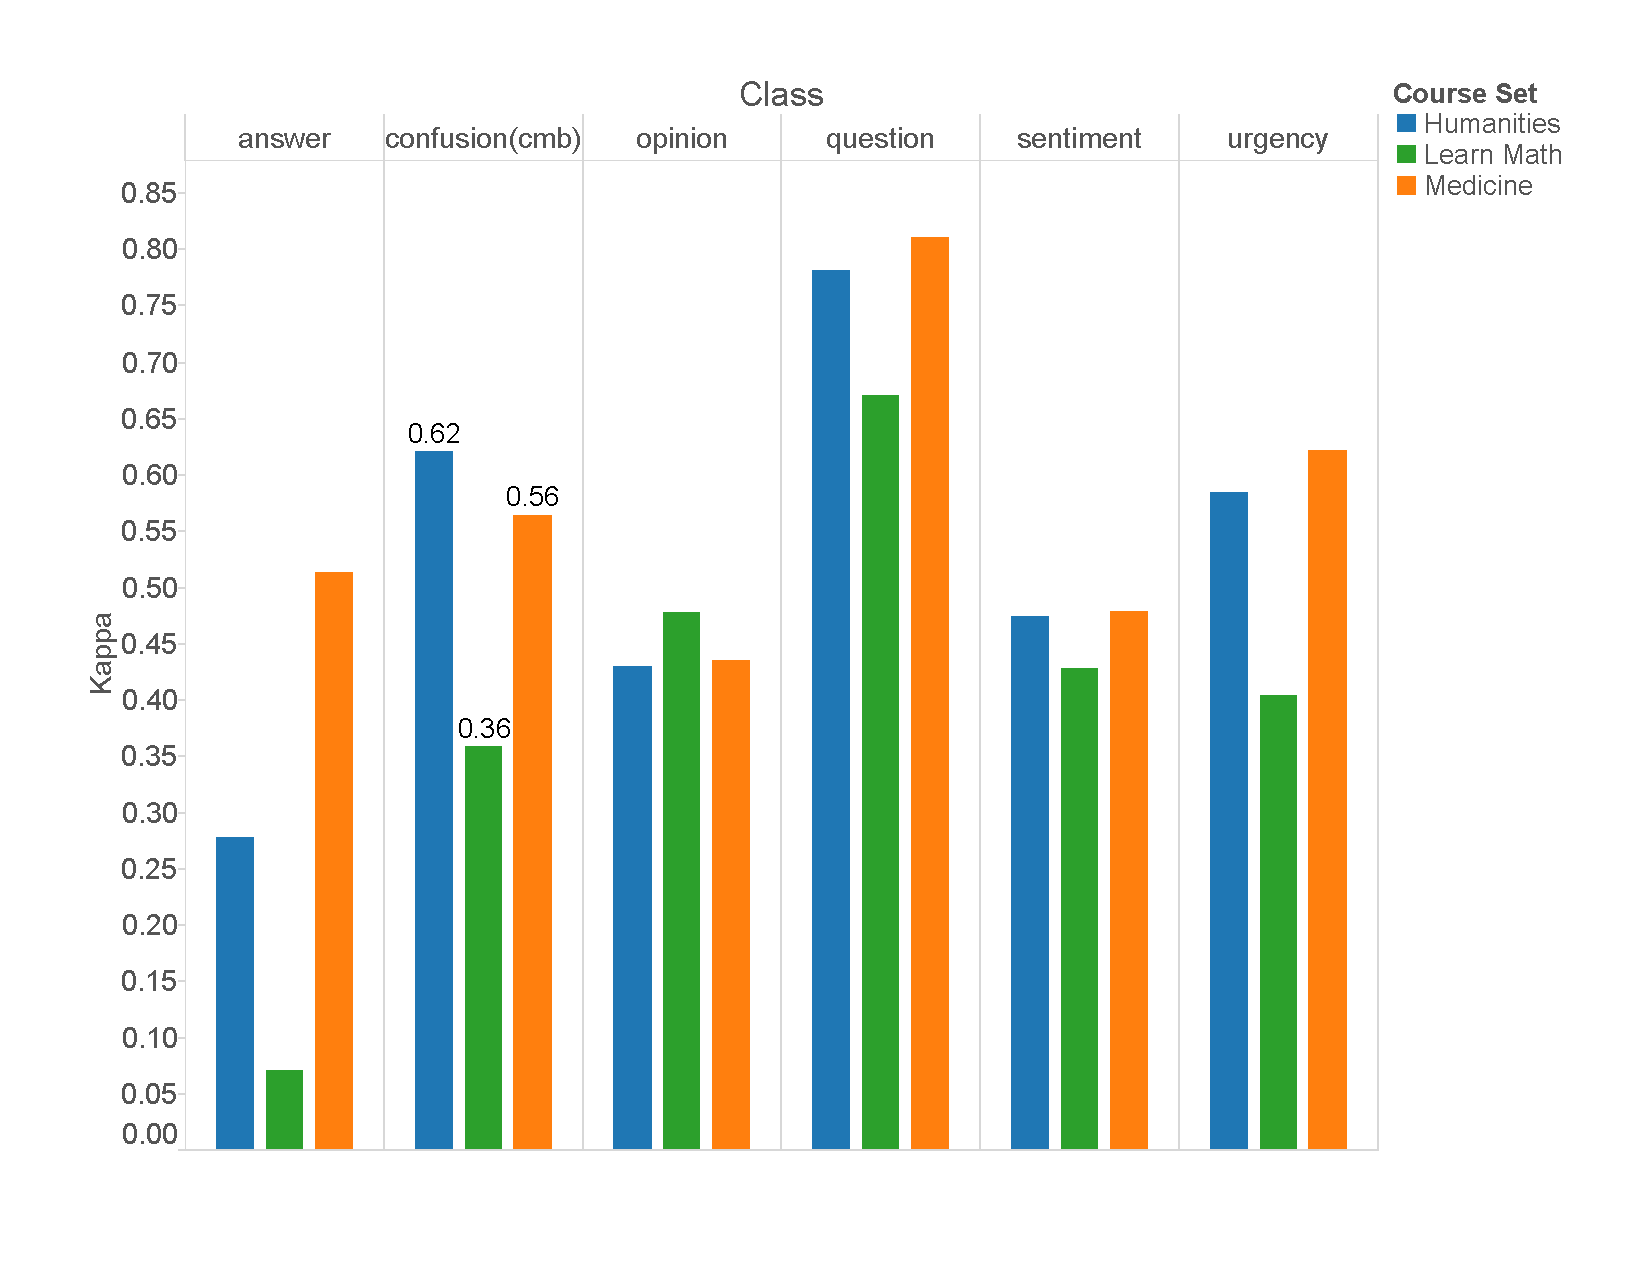
\includegraphics[width=1.0\textwidth]{../Figs/classifierEvalsWithEdu.pdf}
       \caption{\textnormal{Constituent Classifier Performance. Confusion(cmb) is the combined classifier.}}
      \label{figure:constituents}
\end{figure}

The combining function of our combined classifier consistently determined that the constituent classifiers for the question and urgency variables were particularly indicative of confusion (see Table \ref{table:informative_features}). Figure~\ref{fig:ablative} shows the results of an ablative analysis in which one constituent classifier was removed from the combined classifier at a time, until we were left with a classifier with no constituent classifiers (call it a \emph{flat} classifier). The flat classifier performed worse than the combined classifier in the two course sets and the education course. For both course sets, the urgency constituent seemed to be the most helpful of the five constituents---we would expect that instructors would prioritize posts in which learners were struggling to understand the course material. However, the same was not true for \emph{How to Learn Math}, which is consistent with the fact that no significant correlation between confusion and urgency was found (see Section~\ref{sec:MOOCPosts}).

%% \begin{table}[t]
%%        \centering
%%        \begin{tabular}{|c|c|c|c|}
%%        \hline
%%        Course Set           & Humanities & Medicine & Learn Math \\ \hline
%%        Combined Classifier  & 0.621      & 0.564    & 0.359 \\ \hline\hline
%%        Minus Question       & 0.621      & 0.559    & 0.350 \\ \hline
%%        Minus Answer         & 0.620      & 0.555    & 0.345 \\ \hline
%%        Minus Opinion        & 0.619      & 0.553    & 0.310 \\ \hline
%%        Minus Sentiment      & 0.621      & 0.555    & 0.292 \\ \hline
%%        Minus Urgency        & 0.618      & 0.512    & 0.337 \\ \hline
%%        Minus Post Position      & 0.614      & 0.482    & 0.337 \\ \hline
%%        \end{tabular}
%%        \caption{\textnormal{
%%        Ablative Analysis, Kappas. Minus question is the combined classifier without the question constituent; minus answer is minus question without the answer constituent; and so on. 
%%        }} % title of Table
%%        \label{table:ablative} % is used to refer this table in the text
%% \end{table}

\begin{figure}[htp]
       \centering
       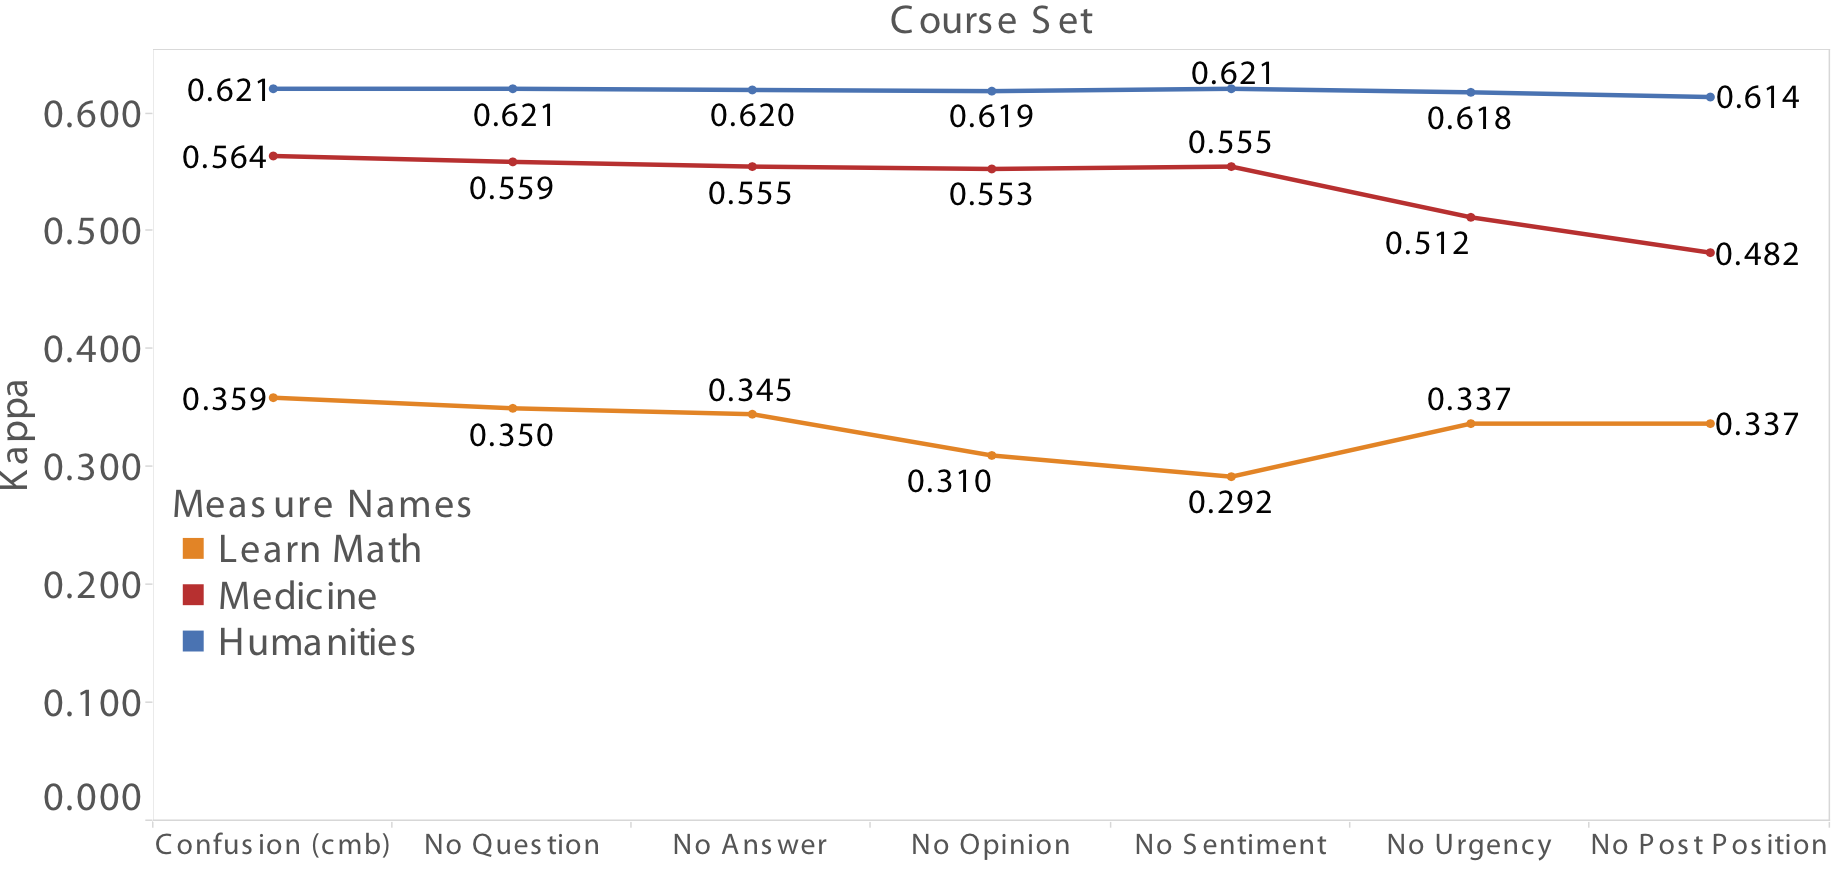
\includegraphics[width=1.0\textwidth]{../Figs/ablativeAnalysisCropped.png}
       \caption{\textnormal{Ablative Analysis, Kappas. No Question
           is the combined classifier without the question
           constituent; No Answer is No Question without the
           answer constituent; and so on.}}
       \label{fig:ablative}
\end{figure}

The post position metadata feature also contributed positively to the classifier's performance---removing it from the flat classifier for medicine dropped the Kappa by 0.03. The other metadata features, however, did not appear to consistently or appreciably affect classifier performance, and so we chose to omit them from our ablative analysis. (Though Table \ref{table:informative_features} shows that the number of question marks was  an informative feature in the \emph{Managing Emergencies} course.)

\section{Phase II: Recommending Clips}
\label{sec:clipRecommendation}
\vspace{1mm}
\subsection{The Recommendation Algorithm}
\vspace{1mm}
In this section, we describe how YouEDU recommends instructional material for a forum post that
has been labelled as \textit{confused} by Phase I. Every course can be thought of as a collection of several video lectures. Each video lecture on average is about 12-14 minutes long. We focus on the problem of identifying a ranked list of snippets, \textit{S}, for each \textit{confused} post. Each snippet \textit{s\textsubscript i} in \textit{S} is a tuple \textit{(video\textunderscore id, seek\textunderscore minute)} where \textit{video\textunderscore id} is an identifier for the recommended video and \textit{seek\textunderscore minute} is the time in the video to which the learner must seek and start playing the video. We would not necessarily need to recommend an \textit{end\textunderscore minute} in a deployed setting (learners could choose when to stop watching).

Phase II of YouEDU is divided into an offline indexing phase and an online retrieval phase.
We define a \textit {bin} as a time-indexed section of a video. Each bin \textit{b\textsubscript{i}} contains the transcribed text content of the video
at a minute-long time interval \textit{i}. We define \textit{binscore(w, b)} of a word \textit{w} and bin \textit{b} as the number of times word \textit{w} appears in bin \textit{b}. We formulate video recommendation to learners as a classical information retrieval problem. In classical IR, the goal is to retrieve the top documents that match a user's query. In our case, the query corresponds to a confused post, and the document corresponds to a bin. We want to retrieve a ranked list of bins that addresses the content of the confused post.

\subsubsection{Offline---Indexing Pipeline}
In the indexing pipeline, we first divide each video into bins. We then use a part-of-speech tagger \cite{nltk} to pre-process each bin. Nouns and noun-phrases tend to produce key-words that typically express what the content is about \cite{hulth2003improved}. Hence, we represent a bin as a triple (\textit{video \textunderscore id}, \textit{start \textunderscore min}, \textit{noun \textunderscore phrase \textunderscore list)} where \textit{noun \textunderscore phrase \textunderscore list} is a collection of only the nouns and noun-phrases in the bin.

We scan through each of the pre-processed bins and build an index from each word to the corresponding bin that the word appears in. This index would enable us to retrieve the list of bins \textit{B\textsubscript{w}}, that corresponds to time epochs in the entire course when the word \textit{w} was discussed. We also maintain a data structure that keeps track of \textit{binscore(w,b)} for every word and bin. The constructed index and data structures are serialized to disk and are used by the retrieval phase.

\subsubsection{Online---Retrieval and Ranking:}
In the online phase, we take as input confused posts. We then use a part-of-speech tagger \cite{nltk} to pre-process each confused post. Similar to the technique we used for bins, we represent each post as a list of its constituent nouns and noun-phrases. Scanning through each of the words in the pre-processed post, we add bin \textit{b} to the candidate set of retrieved bins if at least one term in the pre-processed post was talked about in \textit{b}. Since we have the index constructed offline, we can use it to prune candidates from a large number of available videos (and hence, bins) in the corpus.

We convert each post and bin into a \textit{V} dimensional vector, where \textit{V} is the size of the vocabulary computed over all words used in all lectures of the course. In this vector, the value on the dimension corresponding to word  \textit{w\textsubscript i} is \textit{binscore(w\textsubscript i,bin)}. We define \textit{simscore(P,B)} as the cosine similarity of the post and the bin.
\begin{equation}
simscore(P,B) = \frac{P.B}{\sqrt{\sum\limits_{i=1}^V P_i ^2} \sqrt{\sum\limits_{i=1}^V B_i ^2}  }
\end{equation}
For each candidate bin \textit{C\textsubscript i} in the list of candidates \textit{C}, we compute \textit{simscore(C\textsubscript i, post)}. We rank all bins in C by their \textit{simscore} values and return the ranking.

\subsection{Evaluation}

We evaluated our ranking system on the 2013 run of the \emph{Statistics in
Medicine} MOOC, offered at Stanford University, which had 24,943
learners. We chose a random sample of queries from our MOOCPosts
dataset for that course. We ran each of those posts through Phase I of
YouEDU and chose 20 random posts from the posts that were labeled as
confused. For each of those confused posts our algorithm produced a
list of six ranked video recommendations (that is, six bins, or
one-minute snippets). We then randomized the order within each group
of six, obscuring the algorithm's ranking decisions. Three domain
experts in statistics at Stanford independently evaluated the
relevance of each snippet to its respective post. This process induced
a human-generated ranking, which we then compared to the algorithm's
rank order. The rating scale given to the raters is described
below:

\textit{2:} {\bf Relevant}. The recommended snippet precisely address the learner's confusion.\\
\textit{1:} {\bf Somewhat relevant}. The recommended snippet is somewhat useful in addressing the learner's confusion.\\
\textit{0:} {\bf Not Relevant}: The recommended snippet does not address the learner's confusion.

\subsubsection{Metrics}
We used two metrics to evaluate the relevancy of our recommendations: NDCG and k-precision.

\textit{Normalized Discounted Cumulative Gain (NDCG):}
NDCG measures ranking quality as the sum of the relevance scores (gains) of each recommendation. However, the gain is discounted proportional to how far down the document is in the ranking. The underlying intuition is that the gain due to a relevant document (say, relevance score of 2) that appears as the last result should be penalized more than it would be if it appeared as the first result. Hence, the DCG metric applies a logarithmic discounting function that progressively reduces a document's gain as its position in the ranked list increases \cite{ndcgcite}. The base \textit{b} of the logarithm determines how sharp the applied discount is.

If \textit{rel\textsubscript i} is the gain associated with the document at position i, the DCG at a position i is defined recursively as
\begin{equation}
DCG(i) =
\begin{cases}
rel \textsubscript i & i < b  \\
\ DCG(i-1) + \frac{rel_i}{\log_b{i}} & otherwise \\
\end{cases}
\end{equation}

Since we want a smooth discounting function, we set b to 2. We use a graded relevance scale of 0, 1 and 2, corresponding to the types listed above, and computed the DCG for the ranked recommendations we obtained for each confused post. The ideal value of DCG (IDCG) is defined as the DCG based on the ideal ranking as judged by the raters. To obtain the IDCG, we sort the rankings given by the raters in decreasing order of relevance scores and compute the DCG of the sorted ranking. This corresponds to the maximum theoretically possible DCG in any ranking of the recommendations for that post. We normalize the DCG for our ranking by the IDCG to get the Normalized DCG (NDCG):
\begin{equation}
NDCG(i) = \frac{DCG(i)}{IDCG(i)}
\end{equation}
If there are $n$ recommended documents, then we report\\NDCG(n) as \emph{NDCG}, the overall rating for the ranking. 

\textit{Precision at top k:}
We define the precision of a ranking \textit{R} with \textit{n} recommendations as the fraction of the recommendations that are relevant. The precision at \textit{k} of a ranking \textit{R} is defined as the precision of \textit{R} restricted to its first \textit{k} recommendations. 

\subsubsection{Results}
\begin{table}
    \begin{tabular}{|l|l|l|l|l|}
    \hline
    Rater  & NDCG & k-precision k=1 & k=2  & k=3  \\ \hline
    Rater1 & 0.66 & 0.66            & 0.61 & 0.62 \\ \hline
    Rater2 & 0.90 & 1.0             & 0.97 & 0.97 \\ \hline
    Rater3 & 0.82 & 0.55            & 0.52 & 0.52 \\ \hline
    Avg    & 0.79 & 0.74            & 0.70 & 0.70 \\ \hline
    \end{tabular}
    \vspace{-5pt}
    \caption {NDCG and k-Precision for recommendations}
\label{table:ndcg}
\end{table}

Our results across the raters are summarized in Table \ref{table:ndcg}. Our average precision at k=1 is 0.74. This intuitively means that on 74\% of cases, the first video that we suggest to a learner (as a recommendation for his or her confused post) is a relevant video. The values at k=2 and k=3, at 0.70, are encouraging as well. Our NDCG numbers are high, indicating that we perform relatively well compared to the IDCG.

\section{Future Work}
\label{sec:futureWork}

The work we presented here is a first step; many opportunities for
future work remain. We are actively investigating whether we can
strengthen our video snippet ranking further by considering which
video portions learners re-visited several times. This analysis
catalogs the number of views that occurred for each second of each
instructional video in a course.

Another thrust of future work will use the question and answer
classifiers to connect learners to each other. The challenge
to meet in this work is to identify learner expertise by their answer
posts, and to encourage their participation in answering questions
related to their expertise. As in YouEDU, auxiliary data, such as
successful homework completion, will support this line of
investigation.

A third ongoing project in our group is the development of user
interfaces for both instructors and learners. Using our classifiers,
we have been experimenting with interactive visualizations of our
classifiers' results. The hope is, for example, to have instructors
see major forum-borne evidence of confusion in a single view, and to
act in response through that same interface.

Video recommendations are not the only source of help for confused
learners. Many online courses are repeated during multiple
quarters. It should therefore be possible for our system to search
forum posts of past course runs for answers to questions in current
posts.  Also, not all confusion is resolvable through videos. For
example, difficulties in operating the video player is unlikely to
have been covered in the course videos. Distinguishing such posts is
an additional challenge.

\section{Conclusion}
\label{sec:conclusion}
We presented our two phase workflow that in its first phase identifies
confusion-expressing forum posts in very large online classes. In a
second phase, the workflow recommends excerpts from instructional course
videos to the confused authors of these posts. Our approach utilizes new datasets
of human tagged forum posts, data from learner interactions with online learning
platforms, and video closed caption files that are produced in concert with the
videos for hearing-impaired learners. Evaluations of our classifiers and recommendations show that both phases of YouEDU perform well, and provide insight into the
manifestations of confusion.

As novel online teaching methods are developed, the same underlying
challenges will need to be met: keeping learners engaged, allowing
them to feel like members of a community, and maximizing instructor
effectiveness in the difficult environment of large public classes.
Teaching online to very large numbers of learners from diverse backgrounds is formidable.
But the potential benefits to underserved populations should encourage
the investigative effort required for further research efforts.

\section{Acknowledgments}
We sincerely thank Alex Kindl, Petr Johanes, MJ Cho, and Kesler Tannen
for slogging through the snippet evaluations.

%\end{document}  % This is where a 'short' article might terminate

%ACKNOWLEDGMENTS are optional

% The following two commands are all you need in the
% initial runs of your .tex file to
% produce the bibliography for the citations in your paper.
%\bibliographystyle{abbrv}
%\bibliography{sources}  % sigproc.bib is the name of the Bibliography in this case
% You must have a proper ".bib" file
%  and remember to run:
% latex bibtex latex latex
% to resolve all references
%
% ACM needs 'a single self-contained file'!
%
%APPENDICES are optional
%\balancecolumns
\begin{thebibliography}{10}
\bibitem{stanfordMOOCPosts}
A.~Agrawal and A.~Paepcke.
\newblock The {Stanford} {MOOCP}osts {Dataset}.
\newblock {\url{http://datastage.stanford.edu/StanfordMoocPosts/}}, December
  2014.

\bibitem{glasgow}
I.~R.~G. at~University~of Glasgow.
\newblock Stop word list.
\newblock \url{http://ir.dcs.gla.ac.uk/resources/linguistic_utils/stop_words}.
\newblock Accessed: 2015-02-05.

\bibitem{bennett2005combination}
P.~N. Bennett, S.~T. Dumais, and E.~Horvitz.
\newblock The combination of text classifiers using reliability indicators.
\newblock {\em Information Retrieval}, 8(1):67--100, 2005.

\bibitem{binali2009new}
H.~H. Binali, C.~Wu, and V.~Potdar.
\newblock A new significant area: Emotion detection in e-learning using opinion
  mining techniques.
\newblock In {\em Digital Ecosystems and Technologies, 2009. DEST'09. 3rd IEEE
  International Conference on}, pages 259--264. IEEE, 2009.

\bibitem{nltk}
S.~Bird, E.~Klein, and E.~Loper.
\newblock {\em {Natural Language Processing with Python}}.
\newblock O'Reilly Media, 2009.

\bibitem{boulis2005text}
C.~Boulis and M.~Ostendorf.
\newblock Text classification by augmenting the bag-of-words representation
  with redundancy-compensated bigrams.
\newblock Technical report, University of Washington, 2005.

\bibitem{chaturvedipredicting}
S.~Chaturvedi, D.~Goldwasser, and H.~Daum{\'e}~III.
\newblock Predicting instructor's intervention in {MOOC} forums.

\bibitem{cohen1960coefficient}
J.~Cohen.
\newblock A coefficient of agreement for nominal scales.
\newblock {\em Educational and Psychological Measurement}, 1960.

\bibitem{freeman2004student}
M.~Freeman and A.~Bamford.
\newblock Student choice of anonymity for learner identity in online learning
  discussion forums.
\newblock {\em International Journal on E-learning}, 3(3):45--53, 2004.

\bibitem{Guo:2014:VPA:2556325.2566239}
P.~J. Guo, J.~Kim, and R.~Rubin.
\newblock How video production affects student engagement: An empirical study
  of {MOOC} videos.
\newblock In {\em Proceedings of the First ACM Conference on Learning @ Scale
  Conference}, L@S '14, pages 41--50, New York, NY, USA, 2014. ACM.

\bibitem{hayes2007answering}
A.~F. Hayes and K.~Krippendorff.
\newblock Answering the call for a standard reliability measure for coding
  data.
\newblock {\em Communication methods and measures}, 1(1):77--89, 2007.

\bibitem{hollands2014moocs}
F.~M. Hollands and D.~Tirthali.
\newblock {MOOC}s: Expectations and reality, May 2014.

\bibitem{hulth2003improved}
A.~Hulth.
\newblock Improved automatic keyword extraction given more linguistic
  knowledge.
\newblock In {\em Proceedings of the 2003 conference on Empirical methods in
  natural language processing}, pages 216--223. Association for Computational
  Linguistics, 2003.

\bibitem{ndcgcite}
K.~J{\"a}rvelin and J.~Kek{\"a}l{\"a}inen.
\newblock Cumulated gain-based evaluation of {IR} techniques.
\newblock {\em ACM Transactions on Information Systems (TOIS)}, 20(4):422--446,
  2002.

\bibitem{liu2013sequences}
Z.~Liu, J.~Ocumpaugh, and R.~S. Baker.
\newblock Sequences of frustration and confusion, and learning.
\newblock In {\em Proc. Int. Conf. Ed. Data Mining}, pages 114--120, 2013.

\bibitem{community}
A.~McGuire.
\newblock Building a sense of community in {MOOC}s.
\newblock
  \url{http://campustechnology.com/articles/2013/09/03/building-a-sense-of-community-in-moocs.aspx},
  2013.
\newblock Accessed: 2015-02-01.

\bibitem{Ng:2004:FSL:1015330.1015435}
A.~Y. Ng.
\newblock Feature selection, {$L_{1}$} vs. {$L_{2}$} regularization, and
  rotational invariance.
\newblock In {\em Proceedings of the Twenty-first International Conference on
  Machine Learning}, ICML '04, pages 78--, New York, NY, USA, 2004. ACM.

\bibitem{shaniedurank}
G.~Shani and B.~Shapira.
\newblock EduRank: A collaborative filtering approach to personalization in
  e-learning.

\bibitem{song2007opinion}
D.~Song, H.~Lin, and Z.~Yang.
\newblock Opinion mining in e-learning system.
\newblock In {\em Network and Parallel Computing Workshops, 2007. NPC
  Workshops. IFIP International Conference on}, pages 788--792. IEEE, 2007.

\bibitem{Stephens-Martinez:2014:MMI:2556325.2566246}
K.~Stephens-Martinez, M.~A. Hearst, and A.~Fox.
\newblock Monitoring {MOOC}s: Which information sources do instructors value?
\newblock In {\em Proceedings of the First ACM Conference on Learning @ Scale
  Conference}, L@S '14, pages 79--88, New York, NY, USA, 2014. ACM.

\bibitem{Tomkin:2014:PMU:2556325.2566245}
J.~H. Tomkin and D.~Charlevoix.
\newblock Do professors matter?: Using an a/b test to evaluate the impact of
  instructor involvement on {MOOC} student outcomes.
\newblock In {\em Proceedings of the First ACM Conference on Learning @ Scale
  Conference}, L@S '14, pages 71--78, New York, NY, USA, 2014. ACM.

\bibitem{stanfordDataApps}
S.~University.
\newblock How to access the Stanford Online Learning data.
\newblock {\url{http://vpol.stanford.edu/research}}, 2012+.

\bibitem{Wactlar:1996:IAD:619007.620445}
H.~D. Wactlar, T.~Kanade, M.~A. Smith, and S.~M. Stevens.
\newblock Intelligent access to digital video: Informedia project.
\newblock {\em Computer}, 29(5):46--52, May 1996.

\bibitem{wen2014sentiment}
M.~Wen, D.~Yang, and C.~P. Ros{\'e}.
\newblock Sentiment analysis in {MOOC} discussion forums: What does it tell us?
\newblock {\em Proceedings of Educational Data Mining}, 2014.

\bibitem{wilson1989learning}
N.~Wilson.
\newblock Learning from confusion: Questions and change in reading logs.
\newblock {\em English Journal}, pages 62--69, 1989.

\bibitem{yang2014forum}
D.~Yang, M.~Piergallini, I.~Howley, and C.~Rose.
\newblock Forum thread recommendation for massive open online courses.
\newblock In {\em Proceedings of 7th International Conference on Educational
  Data Mining}, 2014.

\bibitem{wen2015confusion}
D.~Yang, M.~Wen, I.~Howley, R.~Kraut, and C.~Ros{\'e}.
\newblock Exploring the effect of confusion in discussion forums of massive
  open online courses.
\newblock In {\em Proceedings of the Second ACM Conference on Learning @ Scale
  Conference}, L@S '15, New York, NY, USA, 2015. ACM.
  
\end{thebibliography}
\balancecolumns
% That's all folks!
\end{document}
